\documentclass[border=4pt]{standalone}
\usepackage{tikz}
\usetikzlibrary{positioning, arrows.meta, shapes.geometric, calc, fit, backgrounds}
\usepackage{amsmath,amssymb}

\begin{document}
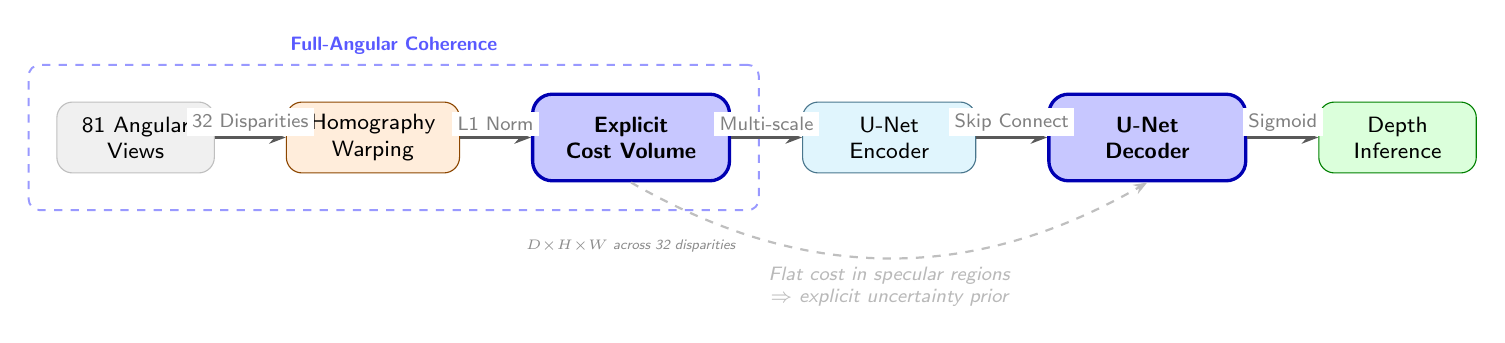
\begin{tikzpicture}[
  input/.style={draw, rounded corners=2mm, minimum width=2.0cm, minimum height=0.9cm,
                fill=gray!12, draw=gray!50, align=center, font=\sffamily\footnotesize},
  proc/.style={draw, rounded corners=2mm, minimum width=2.2cm, minimum height=0.9cm,
               fill=orange!14, draw=orange!55!black, align=center, font=\sffamily\footnotesize},
  module/.style={draw, rounded corners=2mm, minimum width=2.2cm, minimum height=0.9cm,
                 fill=cyan!12, draw=cyan!50!black, align=center, font=\sffamily\footnotesize},
  innov/.style={draw, rounded corners=2.5mm, minimum width=2.5cm, minimum height=1.1cm,
                fill=blue!22, draw=blue!70!black, line width=1.2pt, align=center,
                font=\sffamily\footnotesize\bfseries},
  output/.style={draw, rounded corners=2mm, minimum width=2.0cm, minimum height=0.9cm,
                 fill=green!14, draw=green!50!black, align=center, font=\sffamily\footnotesize},
  arr/.style={-{Stealth[length=6pt]}, thick, color=black!65},
  arrd/.style={-{Stealth[length=5pt]}, dashed, thick, color=gray!50},
  lbl/.style={font=\sffamily\scriptsize, text=black!50, fill=white, inner sep=2pt},
  gbox/.style={draw=blue!40, dashed, rounded corners=4pt, inner sep=10pt, line width=0.7pt},
]

% ---------- Main pipeline (left to right) ----------
\node[input] (m1) {81 Angular\\Views};
\node[proc, right=0.9cm of m1] (m2) {Homography\\Warping};
\node[innov, right=0.9cm of m2] (m3) {Explicit\\Cost Volume};
\node[module, right=0.9cm of m3] (m4) {U-Net\\Encoder};
\node[innov, right=0.9cm of m4] (m5) {U-Net\\Decoder};
\node[output, right=0.9cm of m5] (m6) {Depth\\Inference};

% ---------- Main data-flow arrows ----------
\draw[arr] (m1) -- node[lbl, above] {32 Disparities} (m2);
\draw[arr] (m2) -- node[lbl, above] {L1 Norm} (m3);
\draw[arr] (m3) -- node[lbl, above] {Multi-scale} (m4);
\draw[arr] (m4) -- node[lbl, above] {Skip Connect} (m5);
\draw[arr] (m5) -- node[lbl, above] {Sigmoid} (m6);

% ---------- Auxiliary: uncertainty prior bypass ----------
\draw[arrd] (m3.south) to[bend right=30]
  node[midway, below, font=\sffamily\scriptsize\itshape, text=gray!55,
       align=center, text width=4.4cm, inner sep=3pt]
  {Flat cost in specular regions\\$\Rightarrow$ explicit uncertainty prior}
  (m5.south);

% ---------- Group box ----------
\begin{scope}[on background layer]
\node[gbox, fit=(m1)(m2)(m3),
      label={[font=\sffamily\scriptsize\bfseries, text=blue!65]above:Full-Angular Coherence}] {};
\end{scope}

% ---------- Disparity axis hint under cost volume ----------
\node[font=\sffamily\tiny, text=black!45, below=0.05cm of m3, yshift=-0.55cm, align=center]
  {\textit{$D{\times}H{\times}W$ across 32 disparities}};

\end{tikzpicture}
\end{document}